\section{LEVEL 2 · Spreidingsmaten}

\begin{missie}
Missie: ontdek hoe sterk je data uit elkaar liggen.
\end{missie}

\begin{doel}
\textbf{DOEL} \quad Na dit level kan je:

☐ de \textbf{variatiebreedte} en de \textbf{interkwartielafstand} berekenen en interpreteren;

☐ de \textbf{variantie} en de \textbf{standaardafwijking} berekenen en interpreteren;

☐ het verschil uitleggen tussen een \textbf{steekproef} ($s$, $\overline{x}$) en een \textbf{populatie} ($\sigma$, $\mu$);

☐ twee groepen vergelijken met centrum- én spreidingsmaten.
\end{doel}

\subsection*{Theorie 2.1 · Waarom een gemiddelde niet genoeg is}

Twee thuisverpleegkundigen, An en Bram, besteden gemiddeld allebei 25 minuten per bezoek. Toch is An veel voorspelbaarder: haar bezoeken duren tussen 20 en 30 minuten, die van Bram tussen 10 en 40 minuten. Het \emph{gemiddelde} vertelt je dus maar de helft van het verhaal. Een \textbf{spreidingsmaat} is een kengetal dat weergeeft hoe sterk numerieke data onderling van elkaar verschillen.

\subsection*{Theorie 2.2 · Variatiebreedte en interkwartielafstand}

\begin{theorie}
\begin{itemize}
\item \textbf{Variatiebreedte}: $R=\text{max}-\text{min}$. De afstand tussen het grootste en het kleinste gegeven.
\item \textbf{Kwartielen}: je rangschikt de data en bepaalt de mediaan ($Q_2$). Het \textbf{eerste kwartiel} $Q_1$ is de mediaan van de onderste helft, het \textbf{derde kwartiel} $Q_3$ is de mediaan van de bovenste helft. Bij een oneven aantal gegevens telt de middelste waarde zelf niet mee in de helften.
\item \textbf{Interkwartielafstand}: $\Delta Q=Q_3-Q_1$. Dit is de afstand die de ‘middelste 50 \%’ van de data beslaat.
\end{itemize}
\end{theorie}

\begin{voorbeeld}
\textbf{Voorbeeld.} Zeven peuters hebben er zoveel minuten voor nodig om in te slapen: 12 – 25 – 18 – 9 – 30 – 15 – 21.

Rangschikken: 9 – 12 – 15 – \textbf{18} – 21 – 25 – 30. \quad $\text{Med}=Q_2=18$

Onderste helft 9 – 12 – 15: $Q_1=12$. \quad Bovenste helft 21 – 25 – 30: $Q_3=25$.

$R=30-9=21$ min \quad en \quad $\Delta Q=25-12=13$ min.

\emph{Interpretatie:} de snelste en de traagste peuter verschillen 21 minuten. De middelste 50 \% van de peuters heeft inslaaptijden die tot 13 minuten uit elkaar liggen (van 12 tot 25 minuten).
\end{voorbeeld}

\subsection*{Theorie 2.3 · Variantie en standaardafwijking}

\begin{theorie}
De \textbf{variantie} geeft de spreiding rond het gemiddelde weer. Stappenplan:

\begin{enumerate}
\item Bereken het gemiddelde.
\item Bereken de afwijking van elk gegeven ten opzichte van het gemiddelde: $x-\overline{x}$.
\item Bereken het kwadraat van elke afwijking.
\item Bereken het gemiddelde van die kwadraten.
\end{enumerate}

De \textbf{standaardafwijking} is de positieve vierkantswortel uit de variantie. Zo staat ze in dezelfde eenheid als de data.

\breedtes{40/30/30}
\begin{tabular}{lcc}
\hline
 & populatie (alle $N$ gegevens) & steekproef ($n$ gegevens) \\
\hline
gemiddelde & $\mu=\dfrac{x_1+\dots+x_N}{N}$ & $\overline{x}=\dfrac{x_1+\dots+x_n}{n}$ \\
variantie & $\sigma^2=\dfrac{(x_1-\mu)^2+\dots+(x_N-\mu)^2}{N}$ & $s^2=\dfrac{(x_1-\overline{x})^2+\dots+(x_n-\overline{x})^2}{n-1}$ \\
standaardafwijking & $\sigma=\sqrt{\sigma^2}$ & $s=\sqrt{s^2}$ \\
\hline
\end{tabular}

De steekproefgrootheden $\overline{x}$, $s^2$ en $s$ zijn \textbf{schatters} voor de populatieparameters $\mu$, $\sigma^2$ en $\sigma$.
\end{theorie}

\begin{voorbeeld}
\textbf{Voorbeeld.} Vijf jongeren doen respectievelijk 2 – 4 – 5 – 6 – 8 uur per week vrijwilligerswerk. Dit zijn alle jongeren van de groep (populatie).

\textbf{1.} $\mu=\dfrac{2+4+5+6+8}{5}=5$ uur.

\breedtes{25/25/25}
\begin{tabular}{lcc}
\hline
$x$ & $x-\mu$ & $(x-\mu)^2$ \\
\hline
2 & $-3$ & 9 \\
4 & $-1$ & 1 \\
5 & 0 & 0 \\
6 & 1 & 1 \\
8 & 3 & 9 \\
\hline
\end{tabular}

\textbf{4.} $\sigma^2=\dfrac{9+1+0+1+9}{5}=\dfrac{20}{5}=4$ uur² \quad en \quad $\sigma=\sqrt{4}=2$ uur.

Zouden de vijf jongeren een \emph{steekproef} zijn, dan deel je door $n-1=4$: $s^2=\dfrac{20}{4}=5$ en $s=\sqrt{5}\approx 2{,}24$ uur.
\end{voorbeeld}

\begin{letop}
\textbf{LET OP}

• De som van de afwijkingen $x-\overline{x}$ is altijd 0; daarom kwadrateer je ze eerst.

• De variantie staat in de eenheid \emph{in het kwadraat} (uur²); de standaardafwijking in de gewone eenheid (uur).

• Spreidingsmaten zijn nooit negatief. Zijn ze 0, dan zijn alle gegevens gelijk.

• De interkwartielafstand is de enige spreidingsmaat die weinig last heeft van uitschieters.

• Bij kwalitatieve data kan je geen spreidingsmaten berekenen.
\end{letop}

\begin{ict}
\textbf{ICT-TIP} \quad \emph{Rekentoestel:} STAT $\rightarrow$ 1-Var Stats geeft $\overline{x}$, $\sigma_x$ (populatie), $S_x$ (steekproef), minX, Med en maxX. \emph{Excel:} =GEMIDDELDE(), =MEDIAAN(), =STDEV.P() (populatie), =STDEV.S() (steekproef). De namen kunnen licht verschillen per versie. Controleer altijd of je de populatie- of de steekproefversie nodig hebt.
\end{ict}

\subsection*{Theorie 2.4 · De boxplot}

\begin{theorie}
Een \textbf{boxplot} tekent het vijfgetallenoverzicht: \textbf{min – $Q_1$ – Med – $Q_3$ – max}. De doos loopt van $Q_1$ tot $Q_3$ (dus de lengte van de doos is $\Delta Q$), het streepje in de doos is de mediaan en de snorharen lopen tot min en max.
\end{theorie}

\subsection*{Aan de slag}

\subsubsection*{Oefening 2.1 \quad ★☆☆ \quad Stap voor stap: $R$ en $\Delta Q$}

Acht patiënten wachtten het volgende aantal minuten bij de huisarts: 12 – 3 – 17 – 9 – 5 – 12 – 8 – 6.

\textbf{a)} Rangschik en bepaal min, max en $R$. \lijn

\textbf{b)} Bepaal de mediaan. Verdeel de gegevens in twee helften. \lijn

\textbf{c)} Bepaal $Q_1$, $Q_3$ en $\Delta Q$. \lijn

\textbf{d)} Interpreteer $R$ en $\Delta Q$ in een zin. \lijn

\begin{oplossing}
\textbf{Oplossing 2.1}

a) 3 – 5 – 6 – 8 – 9 – 12 – 12 – 17; min = 3, max = 17, $R=14$ min. b) $\text{Med}=\dfrac{8+9}{2}=8{,}5$ min; helften: 3 – 5 – 6 – 8 en 9 – 12 – 12 – 17. c) $Q_1=\dfrac{5+6}{2}=5{,}5$; $Q_3=\dfrac{12+12}{2}=12$; $\Delta Q=12-5{,}5=6{,}5$ min. d) De langste en kortste wachttijd verschillen 14 minuten; de middelste 50 \% van de wachttijden ligt binnen 6,5 minuten.
\end{oplossing}

\subsubsection*{Oefening 2.2 \quad ★★☆ \quad Variantie en standaardafwijking}

De zes teamleden van een woonzorgcentrum hebben respectievelijk 3 – 5 – 6 – 8 – 12 – 14 jaar anciënniteit. Ze vormen de volledige populatie.

\breedtes{25/25/25}
\begin{tabular}{lcc}
\hline
x & x − μ & (x − μ)² \\
\hline
3 & & \\
5 & & \\
6 & & \\
8 & & \\
12 & & \\
14 & & \\
\hline
\end{tabular}

\textbf{a)} Bereken $\mu$ en vul de tabel aan. \lijn

\textbf{b)} Bereken $\sigma^2$ en $\sigma$ (2 decimalen). \lijn

\textbf{c)} Stel dat de zes teamleden een \emph{steekproef} zijn uit alle teams van de organisatie. Bereken $s^2$ en $s$. Waarom zijn die groter? \lijn

\begin{oplossing}
\textbf{Oplossing 2.2}

a) $\mu=\dfrac{48}{6}=8$ jaar; afwijkingen $-5$, $-3$, $-2$, 0, 4, 6; kwadraten 25, 9, 4, 0, 16, 36 (som 90). b) $\sigma^2=\dfrac{90}{6}=15$ jaar²; $\sigma=\sqrt{15}\approx 3{,}87$ jaar. c) $s^2=\dfrac{90}{5}=18$ jaar²; $s=\sqrt{18}\approx 4{,}24$ jaar. Je deelt door $n-1$ in plaats van $n$: een steekproef onderschat de spreiding van de populatie licht, dat corrigeert $n-1$.
\end{oplossing}

\subsubsection*{Oefening 2.3 \quad ★★☆ \quad Context: wie is het meest voorspelbaar?}

An en Bram (zie theorie 2.1) noteren vijf bezoeken (in minuten):

\breedtes{25/75}
\begin{tabular}{ll}
\hline
verpleegkundige & duur van de vijf bezoeken (min) \\
\hline
An & 20 – 22 – 25 – 28 – 30 \\
Bram & 10 – 15 – 25 – 35 – 40 \\
\hline
\end{tabular}

\textbf{a)} Toon aan dat beide gemiddeld 25 minuten per bezoek besteden. \lijn

\textbf{b)} Bereken voor beide de variatiebreedte en de interkwartielafstand. \lijn

\textbf{c)} Bereken voor beide de standaardafwijking (populatie). \lijn

\textbf{d)} Wie is het best voorspelbaar? Leg uit met je resultaten en schrijf een antwoordzin. \lijn

\begin{oplossing}
\textbf{Oplossing 2.3}

a) $\dfrac{125}{5}=25$ voor beide. b) An: $R=10$, $Q_1=21$, $Q_3=29$, $\Delta Q=8$. Bram: $R=30$, $Q_1=12{,}5$, $Q_3=37{,}5$, $\Delta Q=25$. c) An: $\sigma^2=\dfrac{25+9+0+9+25}{5}=13{,}6$, $\sigma\approx 3{,}69$ min. Bram: $\sigma^2=\dfrac{225+100+0+100+225}{5}=130$, $\sigma\approx 11{,}40$ min. d) An: alle spreidingsmaten zijn veel kleiner, haar bezoeken duren dus steeds ongeveer even lang. Antwoordzin: ondanks hetzelfde gemiddelde is An veel voorspelbaarder dan Bram (σ ≈ 3,69 min tegenover σ ≈ 11,40 min).
\end{oplossing}

\subsubsection*{Oefening 2.4 \quad ★★☆ \quad Koppel: dotplots en standaardafwijking}

Drie groepen van 20 waarden hebben alle drie gemiddelde 20. Koppel elke grafiek aan de juiste standaardafwijking.

\begin{center}
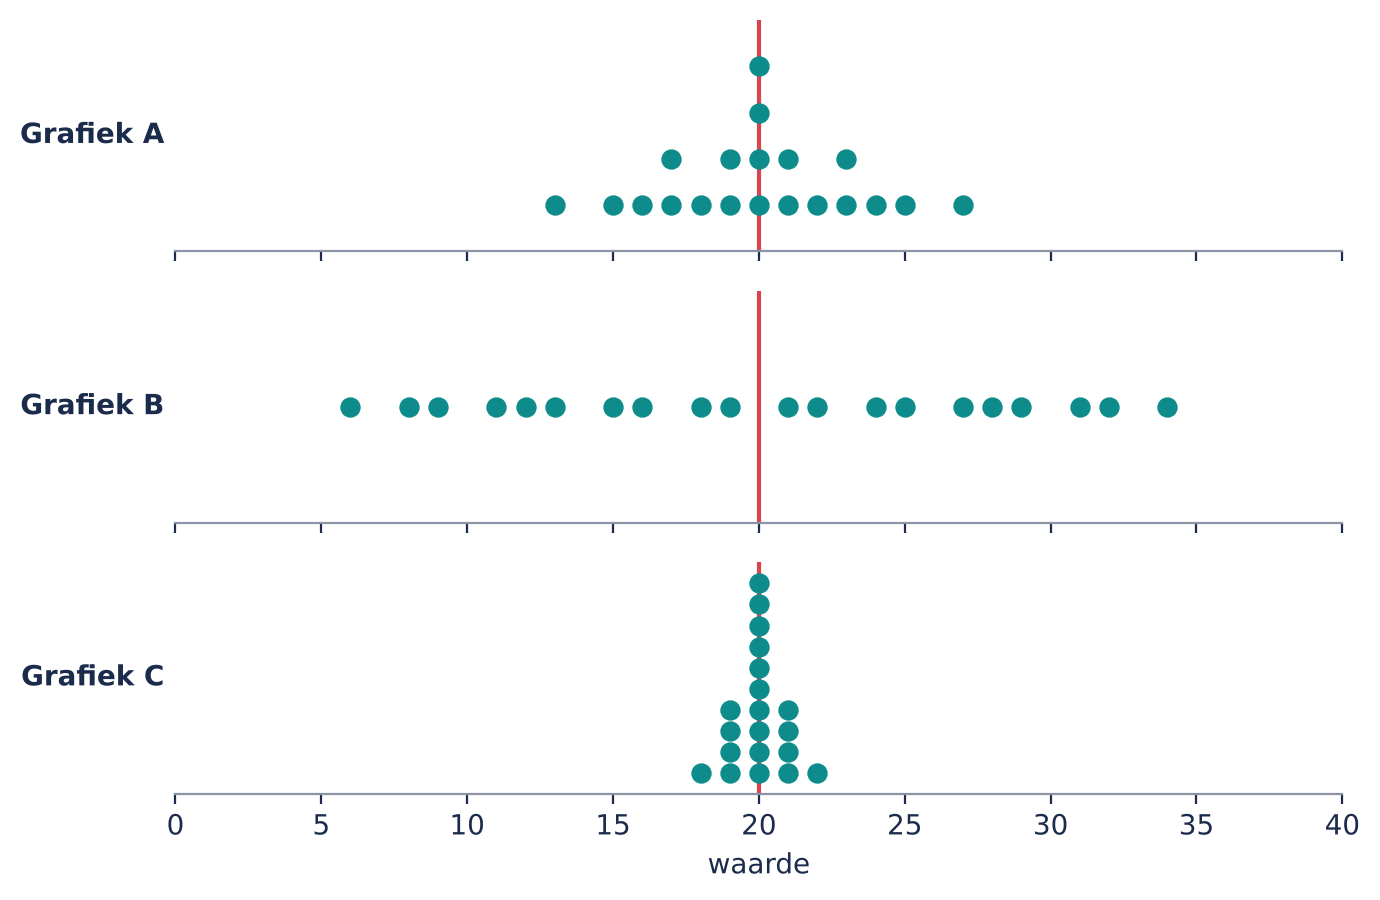
\includegraphics[width=0.8\textwidth]{figuren/l2_dotplots.png}
\end{center}

Standaardafwijkingen: $\sigma\approx 0{,}9$ \quad $\sigma\approx 3{,}4$ \quad $\sigma\approx 8{,}4$

\textbf{Grafiek A:} $\sigma\approx$ \_\_\_\_\_ \qquad \textbf{Grafiek B:} $\sigma\approx$ \_\_\_\_\_ \qquad \textbf{Grafiek C:} $\sigma\approx$ \_\_\_\_\_

\textbf{b)} Welke grafiek heeft de grootste variatiebreedte? Verklaar in één zin. \lijn

\begin{oplossing}
\textbf{Oplossing 2.4}

A: 3,4 \quad B: 8,4 \quad C: 0,9. b) Grafiek B: de punten liggen het verst uit elkaar; hoe groter de spreiding, hoe groter de standaardafwijking.
\end{oplossing}

\subsubsection*{Oefening 2.5 \quad ★★☆ \quad Een boxplot lezen}

Twee klassen noteren hoeveel boeken ze tijdens de vakantie lazen.

\begin{center}
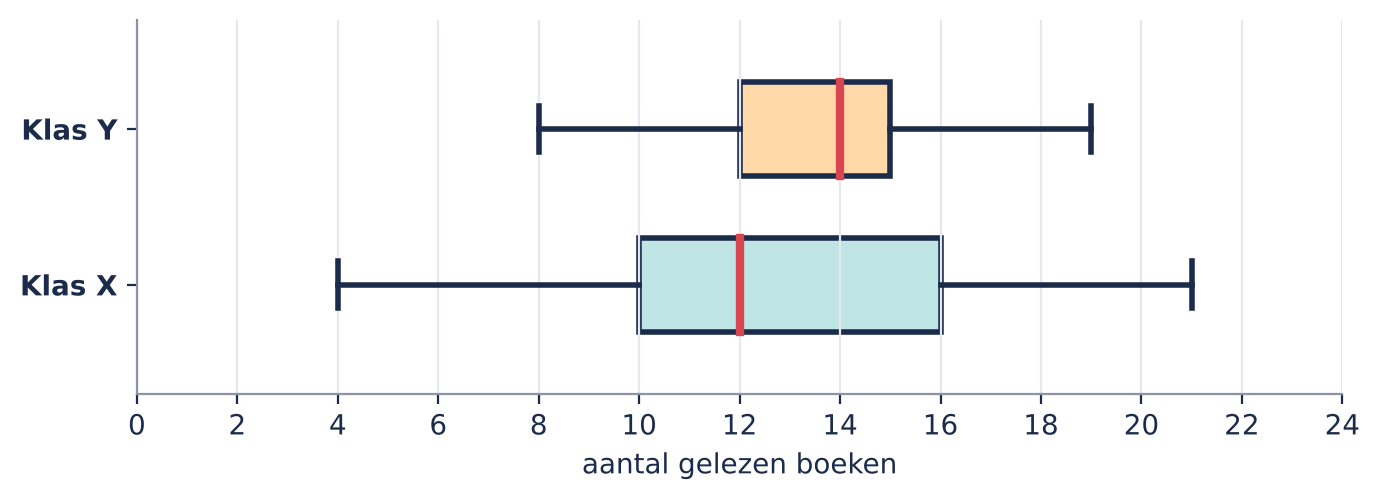
\includegraphics[width=0.85\textwidth]{figuren/l2_boxplot.png}
\end{center}

\textbf{a)} Lees het vijfgetallenoverzicht van beide klassen af. \lijn

\textbf{b)} Bereken $R$ en $\Delta Q$ voor beide klassen. \lijn

\textbf{c)} Welke klas heeft de grootste spreiding? Welke klas leest typisch het meest? \lijn

\textbf{d)} Interpreteer $Q_3$ van klas Y in een zin. \lijn

\begin{oplossing}
\textbf{Oplossing 2.5}

a) Klas X: 4 – 10 – 12 – 16 – 21. Klas Y: 8 – 12 – 14 – 15 – 19. b) X: $R=17$, $\Delta Q=6$. Y: $R=11$, $\Delta Q=3$. c) Klas X heeft de grootste spreiding (zowel $R$ als $\Delta Q$ zijn groter); klas Y heeft de hoogste mediaan (14 tegenover 12). d) Minstens 75 \% van de leerlingen van klas Y las maximaal 15 boeken; ongeveer een kwart las minstens 15 boeken.
\end{oplossing}

\subsubsection*{Oefening 2.6 \quad ★★★ \quad ICT: schermtijd}

Twaalf jongeren noteren hun schermtijd per dag (in uur): 2,5 – 3 – 4 – 1,5 – 5 – 3,5 – 4,5 – 2 – 6 – 3 – 4 – 3,5.

\textbf{a)} Bereken met ICT het gemiddelde en de standaardafwijking, ervan uitgaand dat het een \emph{steekproef} is uit alle jongeren. \lijn

\textbf{b)} Wat is het verschil tussen $\sigma$ en $s$ op je rekentoestel? Welke gebruik je hier en waarom? \lijn

\textbf{c)} Schrijf een antwoordzin waarin je beide resultaten interpreteert. \lijn

\begin{oplossing}
\textbf{Oplossing 2.6}

a) $\overline{x}\approx 3{,}54$ uur en $s\approx 1{,}27$ uur (ter controle: $\sigma\approx 1{,}22$ uur). b) $\sigma$ deelt door $n$ (populatie), $s$ deelt door $n-1$ (steekproef). Hier gebruik je $s$ omdat de 12 jongeren een steekproef zijn. c) De jongeren zitten gemiddeld ongeveer 3,5 uur per dag achter een scherm en de schermtijd wijkt typisch ongeveer 1,3 uur af van dat gemiddelde.
\end{oplossing}

\subsection*{Invullen · de spreidingsmaten}

\textbf{Woordenlijst:} variatiebreedte – interkwartielafstand – variantie – standaardafwijking – nul – uitschieters.

Het verschil tussen het grootste en het kleinste gegeven is de \gat{variatiebreedte}. Het verschil $Q_3-Q_1$ heet de \gat{interkwartielafstand}. De \gat{standaardafwijking} is de vierkantswortel uit de \gat{variantie}. Als alle gegevens gelijk zijn, is de standaardafwijking gelijk aan \gat{nul}. De interkwartielafstand heeft weinig last van \gat{uitschieters}.

\subsection*{Foutjager en redeneren}

\textbf{1.} Jens: ‘De standaardafwijking van mijn data is $-3{,}2$.’ Wat klopt er niet? \lijn

\textbf{2.} Mia: ‘De variantie is 15 jaar.’ Wat klopt er niet? \lijn

\textbf{3.} Alle begeleiders van een team krijgen 2 uur extra per week. Verandert het (ja/nee): gemiddelde, mediaan, $R$, $\Delta Q$, $\sigma$? \lijn

\begin{oplossing}
\textbf{Oplossing Foutjager}

1. Een standaardafwijking is nooit negatief. 2. De variantie heeft als eenheid jaar² (de standaardafwijking is in jaar). 3. Gemiddelde: ja (+2), mediaan: ja (+2); $R$, $\Delta Q$ en $\sigma$: nee, want de onderlinge afstanden blijven dezelfde.
\end{oplossing}

\subsection*{CHECK · Level 2}

Gegeven: 3 – 6 – 6 – 7 – 9 – 10 – 15.

\textbf{1.} (3 p) Bereken de mediaan, $Q_1$ en $Q_3$. \lijn

\textbf{2.} (2 p) Bereken $R$ en $\Delta Q$ en interpreteer $\Delta Q$. \lijn

\textbf{3.} (3 p) Bereken de variantie en de standaardafwijking van de populatie 2 – 4 – 6 – 8 – 10. \lijn

\textbf{4.} (2 p) Twee klassen hebben hetzelfde gemiddelde op een toets, maar klas A heeft $s=3$ en klas B heeft $s=8$. Wat betekent dat? \lijn

\begin{doel}
\textbf{Score:} \_\_\_ / 10 \quad ☐ behaald (vanaf 7 / 10) \quad ☐ nog even oefenen
\end{doel}

\begin{oplossing}
\textbf{Oplossing CHECK 2}

1. Med = 7; onderste helft 3 – 6 – 6 geeft $Q_1=6$; bovenste helft 9 – 10 – 15 geeft $Q_3=10$. 2. $R=15-3=12$; $\Delta Q=10-6=4$: de middelste 50 \% van de gegevens ligt binnen 4 eenheden. 3. $\mu=6$; kwadraten 16, 4, 0, 4, 16 (som 40); $\sigma^2=\dfrac{40}{5}=8$ en $\sigma=\sqrt{8}\approx 2{,}83$. 4. Klas B heeft meer spreiding: de punten liggen verder van het gemiddelde dan in klas A, de resultaten van A zijn gelijkmatiger.
\end{oplossing}
